\documentclass[10pt,a4paper]{article}
\usepackage[utf8]{inputenc}
\usepackage{url}
\usepackage[english]{babel}
\usepackage{amsmath}
\usepackage{amsfonts}
\usepackage{amssymb}
 \usepackage{float}
\usepackage{graphicx}
\usepackage[left=2cm,right=2cm,top=2cm,bottom=2cm]{geometry}
\author{Andres Chaves}
\title{Report 4 }

\begin{document}
 \title{Report 4}
 \author{Andres Chaves (706801) \\
  \multicolumn{1}{p{.7\textwidth}}{\centering{achaves@student.unimelb.edu.au\\}\centering\emph{Melbourne School of Information\\The University of Melbourne}}}
 \maketitle
 
  \begin{abstract}
    The purpose of this document is to continue the analysis of possible algorithms that could help in the analysis of correlation rules for network alarms
\end{abstract}

 \section*{Introduction}
In the last two meetings held, the research problem was further elaborated. It is desired that the outcome of the application of a machine learning algorithm suffices the following requirements:

\begin{itemize}
\item Look at the entire dataset and all alarms types and propose some rules that are useful at suppressing alarms
\item The proposed rules should be as general as possible
\item The algorithm should prefer rules that suppress more alarms.
\end{itemize}

We identified also three types of dependencies between alarms:
\begin{itemize}
\item A large number of low level alarms prior to major failure
\item A fault or situation that causes that some alarms are repeated many times
\item An alarm (root cause) triggers many "symptom" alarms
\end{itemize}

We also analysed the previous data exploration and analysis, which reasoned about the conditional probability of receiving two alarms in a given time window versus the independent probability of each alarm.
\\\\
Additionally, the initial approach suggested a "watch list" of significant alarms in order to constrain the search space and turn the problem feasible.
\\\\
Finally we outlined the plan/questions for the following weeks:
\begin{itemize}
\item Read literature about frequent itemset data mining, specially algorithms that take into account the temporary and the multi-attribute aspects of an alarm.
\item If possible, implement some of the algorithm and analyze the results
\item For the scenario AC Alarm + Link Down analyse what would be the ideal time window size.
\end{itemize}

In the following section we are going to address the result of the planned steps.

\section{Frequent Itemset Mining}
Frequent Itemset Mining attempts to mine association from transactions or datasets. One of the most common applications is Market Basket Analysis, where an Apriori algorithm is used.
\\\\
The inconvenient with the Apriori algorithm is that unlike transaction data, where all items are bought at the same time, alarms include a temporal dimension within. Also, in the Apriori algorithm the name of the items included in the transactions constitutes enough information for the analysis whereas an alarm includes more attributes than just the alarm name, such as hostname or variable bindings.
\\\\
J. L. Hellerstein in his paper "Discovering actionable patterns in event data" discusses some approaches about how the use of frequent item set mining in alarm data. In particular he proposed 4 different strategies for pattern discovery:
\begin{itemize}
\item Event Burst: Correspond to analyse periods where event storms occurs. An event storm is a scenario where one single fail trigger a significant number of symptom alarms.
\item Partially Periodic Patterns: Consist on repeated occurrence of the same alarm set. These periodic behaviour is not necessarily persistent (it may have on and off segments). 
\item Mutually Dependent Patterns: Consist on finding alarm sets where all subsets are significantly dependent.
\item MultiAttribute Pattern Mining: Consist on the use of the multiple attributes that conforms an alarm, such as event name, host name and variable bindings.
\end{itemize}

\subsection{Event Burst}

Event Burst correspond to unusual peaks in the number of events received within a defined window. The algorithm steps for this analysis is the following:

\begin{enumerate}
\item Find periods in which event rates are higher than a threshold
\item Apply Market Basket Analysis of the event names in those periods
\end{enumerate}

Following is the analysis done of event bursts in the testing dataset.
\\\\
We attempted to visually identify patterns in the data and in order to do this we made a hexbin plot of alarm type count vs time:

\begin{figure}[H]
 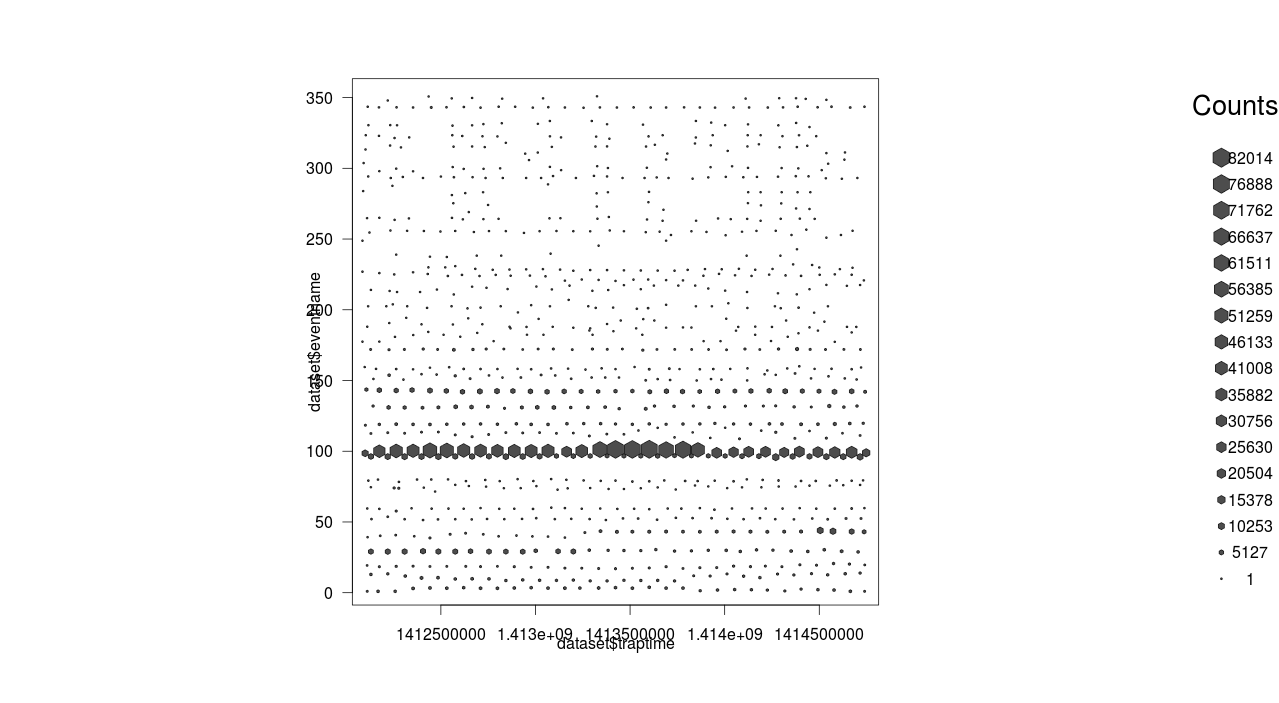
\includegraphics[scale=0.5]{eventHexBin.png}
  \centering
  \caption{\textit{HexBin alarm type vs time }}
  \label{fig:AlarmHexBin}
\end{figure}	

Secondly we charted the frequency of alarms to find unusual counts corresponding to storm of alarms:

\begin{figure}[H]
 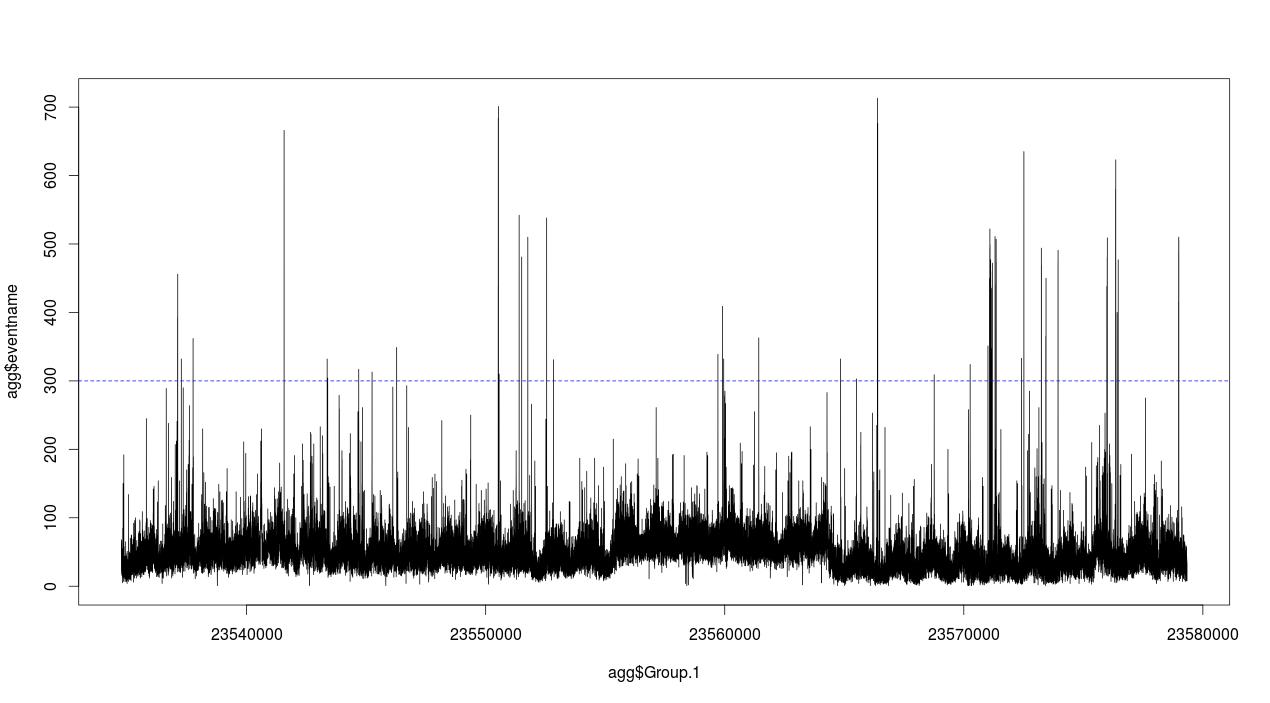
\includegraphics[scale=0.5]{eventBurst.png}
  \centering
  \caption{\textit{HexBin alarm type vs time }}
  \label{fig:EventBurst}
\end{figure}	

We chose the threshold of 300 to declare the time period unusual. There are xx unusual periods in this particular month.
\\\\
Next we executed an Apriori algorithm on the selected time windows. After pruning redundant rules we had 61 rules. We analysed the 61 rules and by domain expert criteria classified them using a is consistent/is not consistent scale, where consistent means whether the association may exist or not. From the 61 rules 7 (11\%) where classified as consistent:

\begin{figure}[H]
 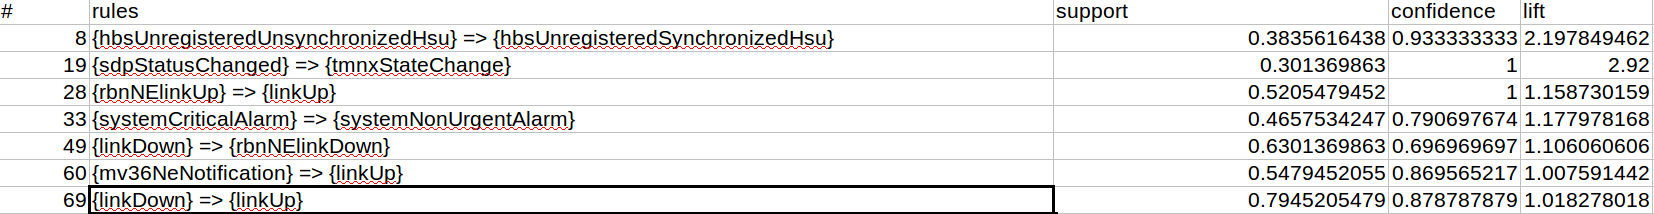
\includegraphics[scale=0.5]{burstRulesEvName.png}
  \centering
  \caption{\textit{HexBin alarm type vs time }}
  \label{fig:EventBurst}
\end{figure}	

We applied the same algorithm again but instead of using alarm names we test the concatenation of alarm name and hostname. After pruning we had 27 rules from which 15 (55\%) where consistent:

\begin{figure}[H]
 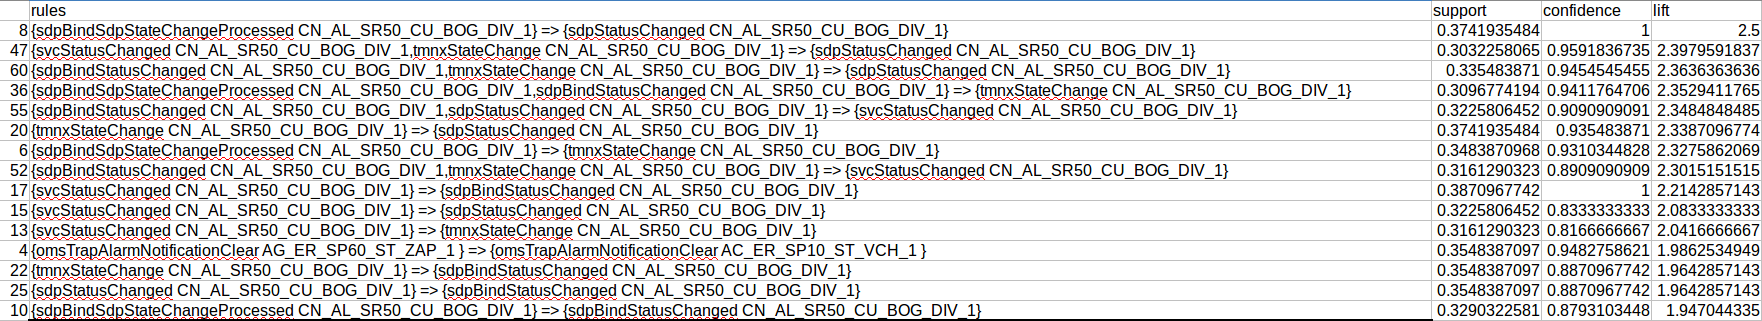
\includegraphics[scale=0.5]{burstRulesEvNameHost.png}
  \centering
  \caption{\textit{HexBin alarm type vs time }}
  \label{fig:EventBurst}
\end{figure}	

It is important to mention that while the former proposed rules cannot be applied directly in a correlation engine they give a good insight on the association between alarms.

\subsection{Partially Periodic Event Patterns}
Partially Periodic Event Pattern mining refers to find periodic event sets that occurs with a given period in segments of the time. Hellerstein addresses this type of data mining in this paper "Mining Partially Periodic Event Patterns With Unkown Periods"\cite{PPatterns}.The algorithm takes into account the following aspects:

\begin{itemize}
\item Periodic behaviour is not necessarily persistent, there are parts of the time where the event set occurs and is periodic and parts where they doesnt.
\item Time may be imprecise.
\item The periodicity is not known in advance.
\item The number of occurrences of a periodic pattern (support) depends on the period.
\item Noise, such as events missing or random events inserted, may be present in the dataset.
\end{itemize}

The algorithm operates in two steps:

\begin{enumerate}
\item Find candidate period lengths for each event type
\item Find temporal associations or P-patterns
\end{enumerate}

In the first step, for each event type the frequency of inter-arrival times is analysed. In this sense bucket counters are created to count the number of occurrences of the event type in the possible periods. Then, to assess if the candidate period is statistically relevant the quantity is tested with a chi-squared method that compares the occurrence with the occurrences generated by a random alarm sequence based on a Poisson distribution.

For the second step, a modified Apriori algorithm is applied. The variations are to take in account time window intervals.

\section{Ideal Time Window for AC + LD scenario}
One of the questions raised in the last meeting was how to estimate  the ideal time window for the AC Outage + LD Scenario. One possible approximation for this is plotting the conditional probability while the window time increases. The following figure illustrates this behaviour:

\begin{figure}[H]
 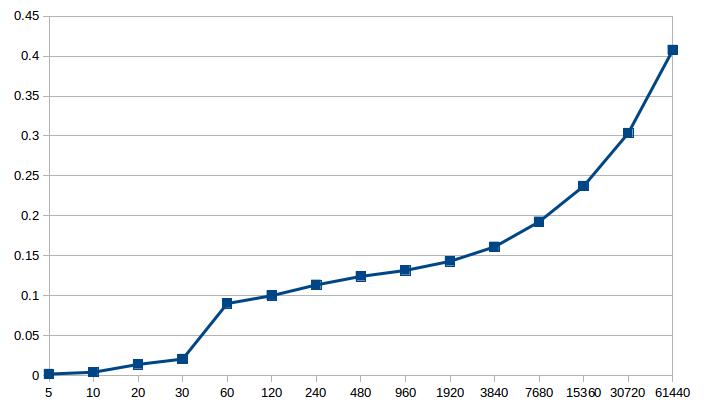
\includegraphics[scale=0.5]{probConditionalScenario.png}
  \centering
  \caption{\textit{HexBin alarm type vs time }}
  \label{fig:ProbCond}
\end{figure}	


 \begin{thebibliography}{9}
\bibitem{discoveringPatternsInEventData} Hellerstein, J. L. and Ma, S. and Perng, C.-S., \emph{Discovering Actionable Patterns in Event Data}.
        IBM Syst. J. 41, 3 (July 2002), 475-493.
\bibitem{PPatterns} Sheng Ma and Joseph L. Hellerstein., \emph{Mining Partially Periodic Event Patterns with Unknown Periods}. Proceedings of the 17th International Conference on Data Engineering (2001). IEEE Computer Society, Washington, DC, USA, 205-214..
\end{thebibliography}
 \end{document}